\chapter{Results and Discussion}

\section{Piezo1 as integrator of biomechanical events in MSCs}
\label{sec:piezo1-as-integrator-of-biomechanical-events-in-mscs}

\myworries{How does the peak relate to flow rate? Is there saturation?}
It is well known, that stem cell migration, differentiation and self-renewal is significantly influenced by physical interaction between the cell, its surrounding microenvironment and exogenous forces. \cite{Eyckmans2011, Lee2011}]MSCs are arguably the most thoroughly studied type of stem cell in this context, possibly because of the promising potential they hold for regenerative medicine and relative ease of access. Extensive studies of different force parameters (e.g. type, amplitude, static/dynamic) on MSCs give great insight into pathways mediating mechanotransduction and guiding the cells behaviour. However, the significance of \Piezo{} and the associated calcium-ion influx in MSC mechanosensing is not fully understood. In the following part we want to elucidate whether \Piezo{} is functionally able to elicit a significant intracellular signal in MSCs that can be classified as mechanotransductory significant.\\
In a reductionist approach, we conclude a relevant contribution of \Piezo{} if we are able to show that MSCs exhibit a \Piezo{}-mediated influx of extracellular calcium ions in response to mechanical force.\\
For our first experiment, Flowchambers were prepared with wild-type (WT) cells being seeded and stained as described in \vref{sec:FluidicModel}. For each flowchamber two separate calcium imaging recordings were carried out in close temporal sequence to each other: The first recording was done using the previously mentioned flow rate protocol executed with modified, calcium-free ACSF as flow shear medium. Upon completion of the first recording, the flow shear medium is exchanged for normal, calcium containing ACSF and the cells continuously flushed for 12 minutes with a total volume of 2.4 ml. After the flushing period, a second recording was done with the previously used flow rate protocol but this time with normal ACSF. After both measurements were completed, the integrity of the flowchamber was assessed by eye and the recordings deemed qualified for analysis, when no violation of structural integrity was observed. The sequence of first calcium-free and second calcium-containing medium is important, as reactive capability of the cells has to be demonstrated in the last measurement to rule out cell death as a possible explanation for lack of impulse response. We then concatenated the two measurements and let them \myworries{!finish at home, explain code pipeline}. We saw a maximum increase of up to 80\% in fluorescence signal in direct response to shear pulse as opposed to no or slightly negative pulse response in the calcium-free measurement. While the amplitude is likely a function of intracellular state, laminar flow defects and flowchamber and grating specific random errors, thus varying over different biological donors, we still see a clear-cut necessity of extracellular calcium-ion presence for successful impulse response. Surprisingly, the shear flow pulse seems to have a negative effect on fluorescence levels of the cell, as illustrated by the bump \myworries{Fig Reference}. We argue that this is likely a technical issue resulting from a combination of loosely-adherent highly fluorescent particles segmented as a cell and the static nature of our segmentation method. During the flow pulse, the particles are swept away, leaving only non-fluorescent substrate and thus leading to an incorrect classification of a decrease in fluorescence. A second technical issue is the discontinuity in apparent fluorescence between the two measurement, with the second measurement starting shy above a ratio of one. We argue this is due to the calcium-starved cell increasing the calcium-influx after resupplying them with extracellular calcium-ions during the flushing period. As this bias corresponds to maximally \myworries{XX}\% of the fluorescence response, we did not correct for this error. Another minor technicality is the slightly negative slope of the baseline. This corresponds to the known property of fluorescent markers to decrease in fluorescence as a function of light exposure, and is called Photobleaching. As the effect is likely neglibible, it is still important to keep in mind, that the signal in the second measurement likely would be slightly higher, since it has the added effect from the first measurement's photobleaching.

\begin{figure}
\centering
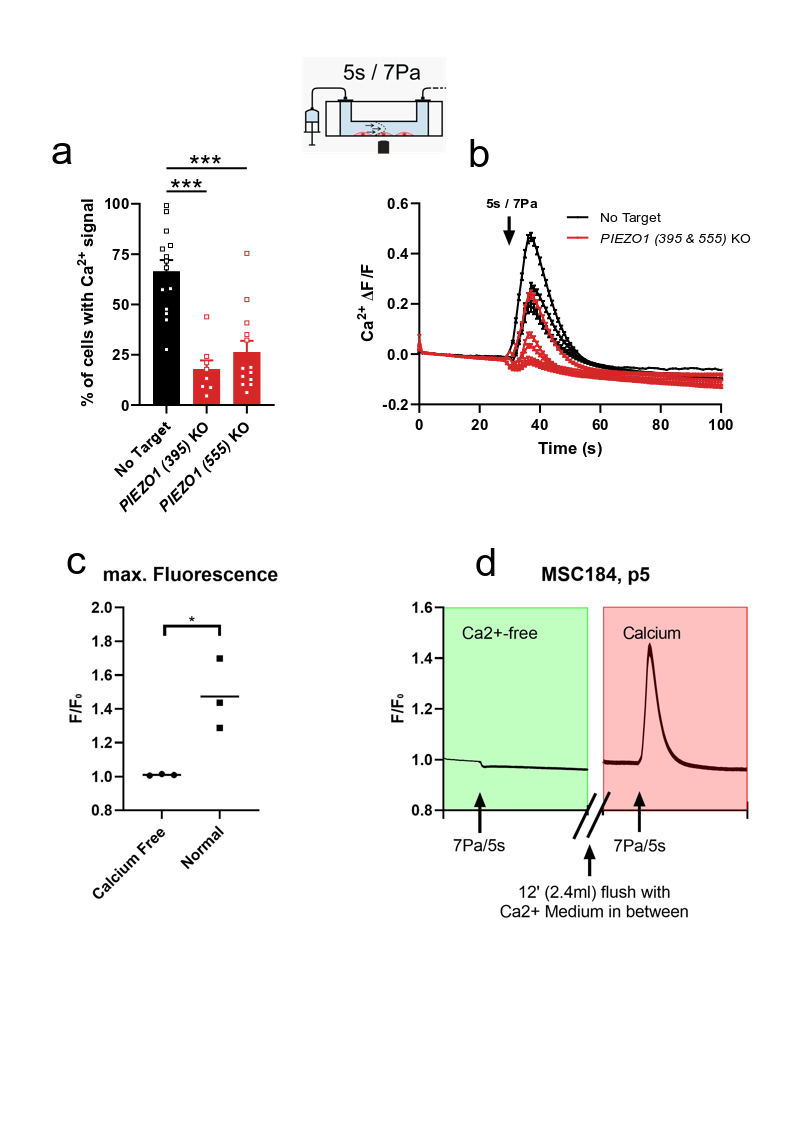
\includegraphics[width = 0.7\textwidth]{Combined_CalciumFree_KnockOut.png}
\caption{Piezo1-mediated influx of extracellular Ca2+ confirmed as mechanotransductory event in MSC. \hfill \newline 
\textbf{a.)} Representative fluorescence level measurement of impulse response with two different media where arrows mark the start of a 7Pa shear stress period of 5s. (Pooled data of 4 technical replicates, Data is mean $\pm$ SEM)	
\textbf{b.)} Peak values of fluorescence levels of samples in calcium-free and calcium-containing medium. (n = 3, *p $<$ 0.05, Student's t-test) 
\textbf{c.)} Temporally resolved fluorescence Signal of Piezo1-KO Cells compared to Control in response to 7 Pa shear period of 5s as denoted by arrow.  
\textbf{d.)} Relative amount of cells that showed fluorescence level impulse response. (Data points describe technical replicates, ***p$<$0.0001, ANOVA with Dunnette's multiple comparison test)}
\label{fig:CalcImaging_Cells}
\end{figure}

We demonstrated that MSCs exhibit reactive mechanosensitive capabilities through force-mediated rapid onset influx of extracellular calcium-ions. The role of \Piezo{} in this process, however, is not defined. To shed light on the contribution size of \Piezo{} we compared the impulse response capabilities of two distinct \Piezo{}-knock out constructs to a control cell line.\\
In preparation for this experiment three transfected cell lines were generated (2 distinct \Piezo{} knock-out's and one negative control) using pre-made lentivirus, carrying a CRISPR/Cas9-system with puromycin resistance as the selection marker. The grouping is specified through the Lentiviral Construct used, resulting in cell line P1-395 (Deletion at \myworries{Ask MATTHIAS}), P1-555 and NoT (No Target, Control for the viral treatment with no putative genome mutation).  In order to assess knock-out efficiency, both Western Blot and qRT-PCR were done not more than one passage after thawing, to avoid overestimation of knock-out efficiency as it likely increases with growing passages. With an knockout efficiency on mRNA-level of XX\% in P1-395 and XX\% in P1-555 and a corresponding knockout-efficiency on protein-level of XX\% in P1-395 and XX\% in P1-555, respectively, we can consider this cell line a valid knock-out model. \myworries{Add efficiency numbers of knockout} 

We then seeded cells in flowchambers and measured the intracellular calcium signal of the cells in response to a shear pulse, similar to the protocol from the previous experiment but only with a single measurement per flowchamber with normal ACSF as shear flow medium. Intriguingly, the knock-out cells show a significantly reduced reaction capability when compared to control. \myworries{FigReference} When comparing the relative amount of knock-out cells that exhibit calcium-influx in response to shear stress, we see a 66\% decrease compared to control, with the effect being bigger in P1-395 (-73\%) as in P1-555 (-60\%). Interestingly, this difference between two different constructs regarding their reduction of impulse response correlates with the knock-out efficiency. Figure 3.b, which shows the same data, but over full temporal resolution, illustrates how the area under the curve is largely reduced when \Piezo{} is knocked out. Modelling of the channel dynamics using a simple statistical model shows that, the decay mechanics largely stay the same with only the amplitude changing to lead to this result, or differently put: The model suggests that there is no compensating adaptation of single channel mechanics in response to lower channel abundance.

These results confirm that \Piezo{} is the main driver in force-mediated calcium-influx in mesenchymal stem cells.


\section{Piezo1 and the extracellular matrix}
\label{sec:PiezoandECM}


\begin{figure}[ht]
	\centering
	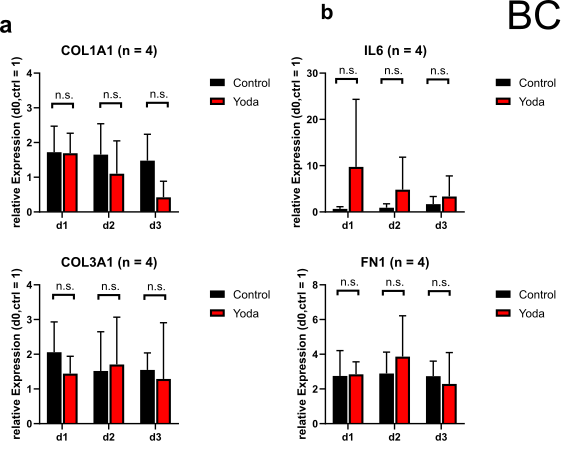
\includegraphics[width = 0.7\textwidth]{NormalYodaExp_PCR.png}
	\caption{mRNA levels of selected gene products after 30min chemical stimulation of \Piezo{}, harvested after 24, 48 or 72 hours, denoted by d1, d2 or d3, respectively. Normalized against d0, control.\hfill \newline
		\textbf{a.)}: \colone{}
		\textbf{b.)}: IL-6
		\textbf{c.)}: \colthree{}
		\textbf{d.)}: \textsc{Fn}1. 
		(Student's t-test with Holm-Sidak multiple comparison correction, n = 4). 
	}
	\label{fig:Yoda_Norm_PCR}
\end{figure}




Preliminary mass spectroscopy secretome analysis of \Yoda-treated cells showed a distinct decrease in core extracellular matrix (ECM) components, such as alpha-1 type I collagen (\colone), Fibronectin-1 (\textsc{Fn1}) and finally alpha-1 type III collagen (\colthree) (Not shown here). This inspired further investigation into this matter.\par



After seeding cells in serum-free medium and letting them rest, we chemically stimulated \Piezo{} with \Yoda{} during 30 minutes, before washing them and transferring them in the incubator again, following the protocol described earlier ~\vref{sec:ChemicalStimulation}. We then harvested identical samples right after intervention (d0) and after 24, 48 and 72 hours (denoted d1, d2 and d3, respectively) to achieve temporal resolution. There were minor loading problems during Western Blotting, but we concluded them to be valid as they did not affect the central tendency of our data. \par

\begin{figure}[htbp]
	\centering
	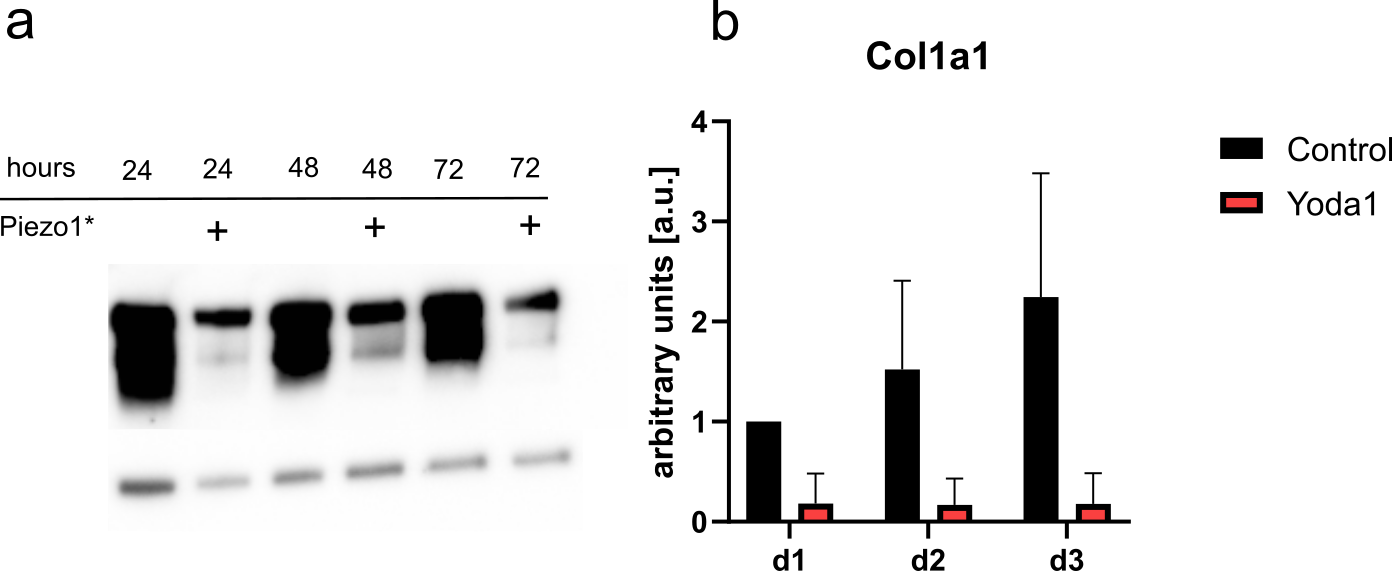
\includegraphics[width = 0.7\textwidth]{NormalYodaExp_WesternBlot_Col1a1.png}
	\caption{
		\textbf{a.)} Representative Chemiluminescence for \colone with control and chemically stimulated \Piezo{}-samples with alpha-Tubulin as housekeeper.
		\textbf{b.)} Quantification of repeated experiments, each data point normalized against housekeeping protein (loading correction) and corresponding d1, control-sample (donor-specific correction).}
	\label{fig:Yoda_Norm_WB}
\end{figure}

\begin{figure}
	\centering
	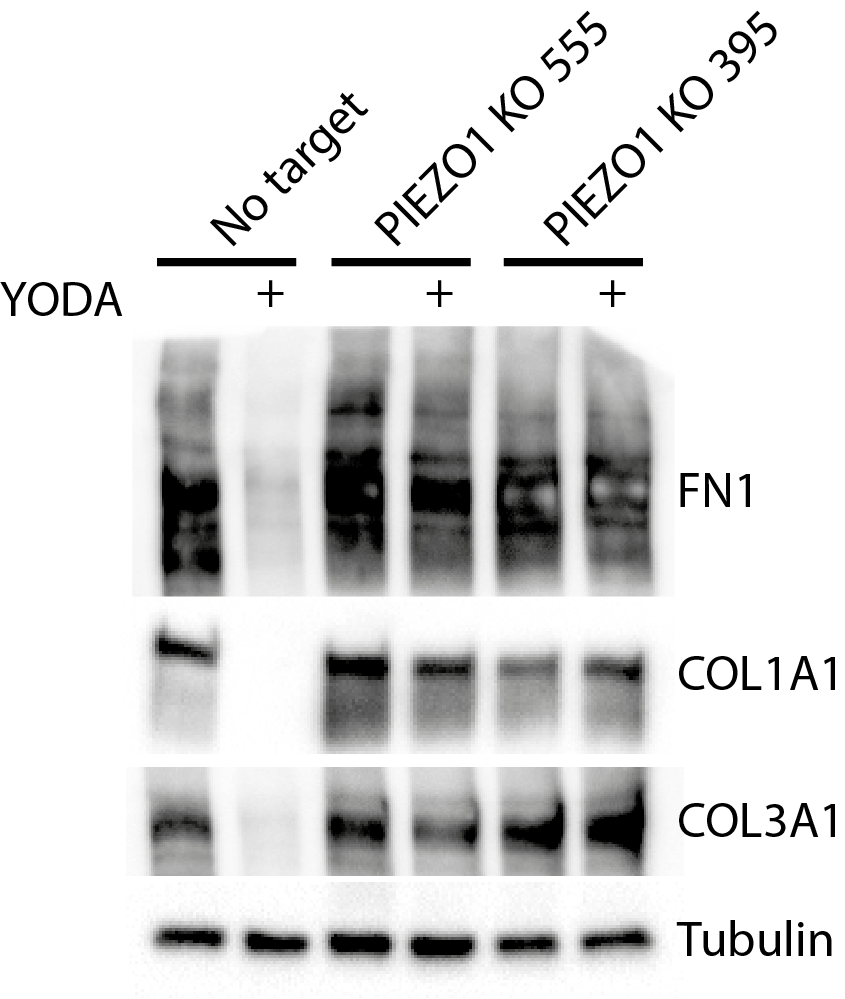
\includegraphics[width=0.7\linewidth]{Uli_Blot_KO.png}
	\caption{Western Blot of selected ECM components comparing protein content of different cell lines 3 days after 30min exposure to either MEM\textalpha{} only (negative control) or MEM\textalpha{} supplemented with 5\textmu{}M chemical \Piezo{} agonist (YODA +), \textalpha{}-Tubulin as housekeeping protein. (n=3, Student's t-test)
	}
	\label{pic:UliBlot}
\end{figure}

Western Blot Analysis of intracellular protein showed a trend of declining \colone-content in samples that have been treated with \Yoda{} (As shown in \ref{fig:Yoda_Norm_WB}). Furthermore, the effects were not only marked by fast onset but also of long-lasting nature, since the effect of a singular 30 minutes \Yoda{}-exposition remained the same three days after intervention. This effect can also be seen in \textsc{Fn1} and \colthree{} (see ~\vref{pic:UliBlot}.) \par

Using qRT-PCR, we also looked at mRNA representation while biasing our investigation towards \colone{}, \colthree{}, \textsc{Fn}1 and Interleukin-6 (IL-6) with GAPDH and RPL13A as house-keeping genes. All measurements were normalised against negative control samples harvested immediately after the intervention. \\
IL-6 results are inconclusive because of the big variance. However, there is a trend of an increase in \Yoda{} samples at d0 followed by a relaxation over following three days to near-normal levels. This strong response is interesting, but it remains to be investigated, whether this translates to a \textit{de facto} increase in IL-6. mRNA levels of \colone{} show a decreasing trend over time, while \colthree and \textsc{Fn}1 stayed largely the same (see Fig. \ref{fig:Yoda_Norm_PCR})\\\par

Interestingly, the trend of \colone{}, \colthree{} and \textsc{Fn1} being largely reduced on protein level is not reflected by the mRNA representation. Since mRNA levels are unchanged and secretome analysis reflects the decrease, the effect of the intervention must act between transcription of mRNA and secretion of the protein. \\
ECM components are known to be post-transcriptionally modified both in the ER and in the endosomal compartments, which are the transporter entities involved in the secretion \cite{Ishida2011, Zeltz2014}, which makes additional studies necessary for more sophisticated hypothesis. One straightforward explanation for the observation could be calpain, a protease that relies on calcium as a cofactor for effector function \cite{Goll2003}. McHugh and colleagues produced evidence for calpain being a downstream effector of \Piezo{} \cite{McHugh2010}. Furthermore, there are studies that link calpain activity to skin wound healing, which is heavily dependent on ECM and specifically \colone{} \cite{Nassar2012}. However, in this paper, Nassar and colleagues demonstrate that calpain-inhibition leads to reduction of \colone{} mRNA, which implicitly contradicts this data. To further investigate this dynamic, it might be worthwhile to investigate the relationship between \Piezo{}-dependent calcium influx and subsequent activation of calpain. \par

One important thing to keep in mind is the design of this study. Cells were previously cultured with 5 \textmu{}g/ml FGF-2 and 10\% FBS, before they were serum-starved and FGF-2 deprived for the experiment. This likely leads to confounding factor including differentiation, which would have to be addressed in future studies.\par

In conclusion, this divergence between decreased protein with largely normal mRNA levels as a consequence of \Piezo{}-stimulation introduces a new dimension, inspiring further research into the topic.

\section{Reversibility and osteogenic differentiation}

\begin{figure}[ht]
	\centering
	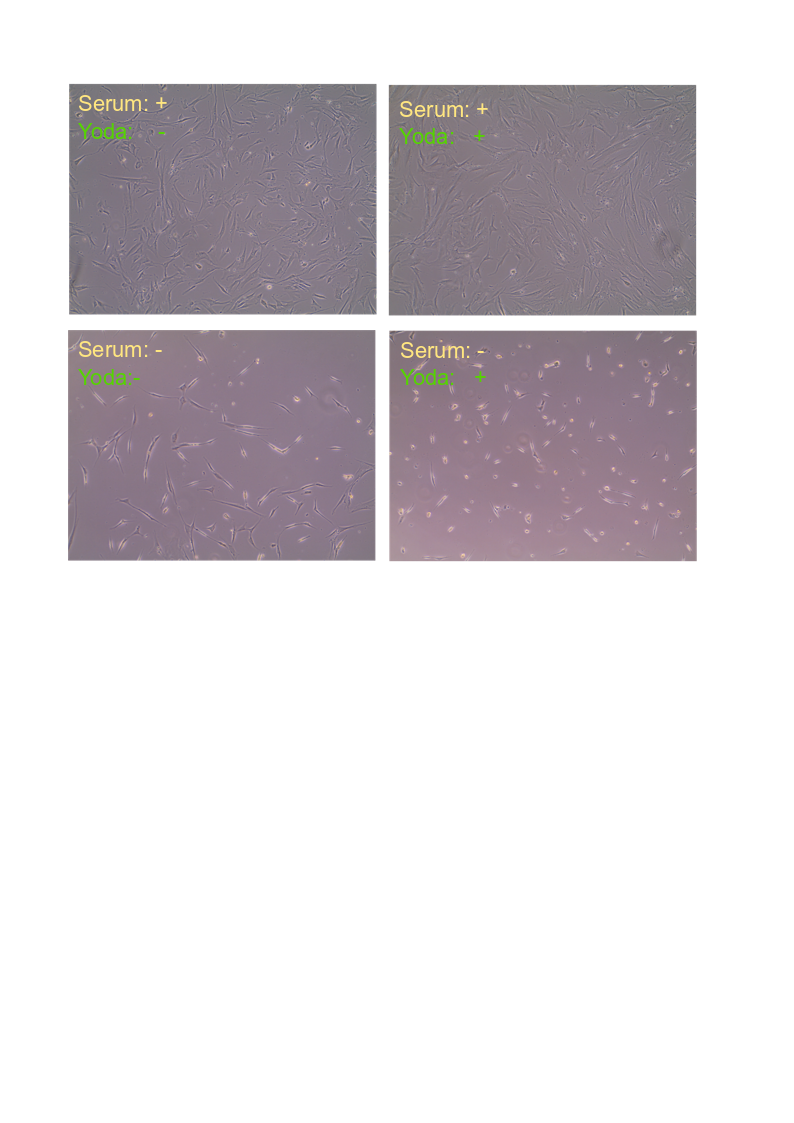
\includegraphics[width = \linewidth{}]{LongTerm_CellPicture.png}
	\caption{
		Light microscopy picture taken of cells seven days after 30min intervention with either  0\textmu{}M (Yoda: -) or 5\textmu{}M (Yoda: +) chemical \Piezo{}-agonist. Three days after intervention, medium was replaced with either serum-free MEM\textalpha{} (Serum: -) or MEM\textalpha{} supplemented with 10\% FBS (Serum +).}
	\label{pic:Cells_LongTerm}
\end{figure}

\begin{figure}
	\centering
	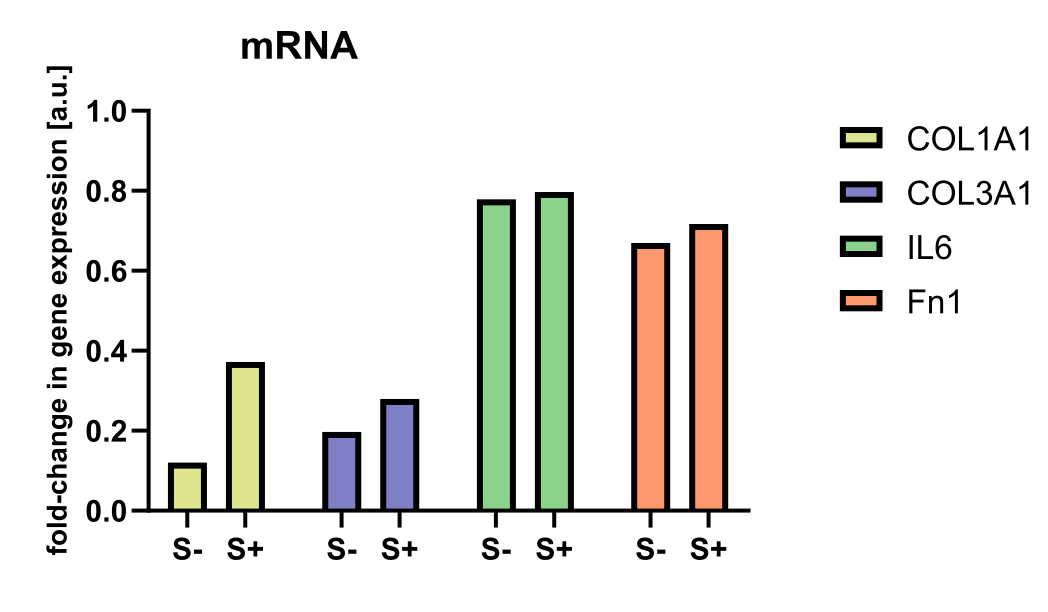
\includegraphics[width = \linewidth{}]{LongTerm_PCR.png}
	\caption{mRNA transcript levels of samples that have been harvested seven days after 30min 5\textmu{}M Yoda exposure normalized against corresponding negative control also from seven days post intervention. We changed the media three days after \Yoda intervention and supplemented the MEM\textalpha{} with either 0\% (Serum -) or 10\% FBS (Serum +). (n = 1)}
	\label{fig:LongTerm_PCR}
\end{figure}

As we saw that intracellular \colone{} protein levels did not recover during our previously chosen timeframe, we wanted to investigate whether the cells would reach a pre-intervention homeostatic state after a longer duration. For this reason, we decided to repeat the experiment from before, but only harvesting the cells after seven days (168 hours). Because in the experiment before we qualitatively saw a steady decrease in cell viability, as assessed by morphological changes in \Yoda{}-treated samples (see on page \pageref{pic:Yoda_Apop}), we adapted the protocol to improve cell viability. In order to allow for sufficient cell survival until cell harvesting, the medium was changed three days after the intervention. Half of the cells received serum-free MEM\textalpha{} (Group denoted by S-), whereas the other half was administered MEM\textalpha{} with 10\% FBS (denoted by S+). For this experiment we only did qRT-PCR, since we were technically limited due to very low yield in the S-/Y+ - group. All samples were normalized against negative control samples from day 7.\\
Interestingly, in our experiment the RNA levels of \colone{} was still drastically lowered independent from FBS supplementation, with as low as 12\% in the serum-starved group. While \colthree{} was also low, this could also be explained by a great variance, which we saw in the experiment before (see Fig. \ref{fig:Yoda_Norm_PCR}). IL-6 and \textsc{Fn}1 was slightly reduced. It is important to keep in mind, due to the experiment being a single measurement, this qualifies only as an exploratory experiment at best.\\
However, there are some plausible indications. For example, it is interesting to note, that IL-6 recovered completely to pre-intervention level, as implied in the experiment before. \\
Furthermore, when looking at \colone{} in serum-suplemented samples, while the PCR levels remained low (~ 30\% of negative control), the cells proliferated and seemed "happy". This implies that \Piezo{}-mediated apoptosis and downregulation of ECM components are mediated by two independent pathways, both downstream of \Piezo{}, as the apoptosis-effect discussed in the next chapter is neutralized by addition of FBS, whereas the downregulation of \colone{} seemingly is not.\\
One alternative explanation would be that the applied \Yoda{}-stimulus leads to a persistent change and possibly to differentiation.\par

Sugimoto and colleagues suggested that \Piezo{} activation leads to osteogenic (meaning bone-like) differentiation \cite{Sugimoto2017}. To test whether we reproduced their results by \Piezo{}-activation, we employed the same protocol, consisting of 30min 5\textmu{}M \Yoda{} intervention with the only experimental samples from day 3, which then are normalized against negative control samples harvested right after the intervention. As read-out method we chose qRT-PCR, following Sugimoto's paper, and biased our analysis against both early osteogenic genes like RUNX2 and late osteogenic genes like ALPL and SPP1 \cite{Marom2005, Creecy2013}. \par


\begin{figure}[htbp]
	\centering
	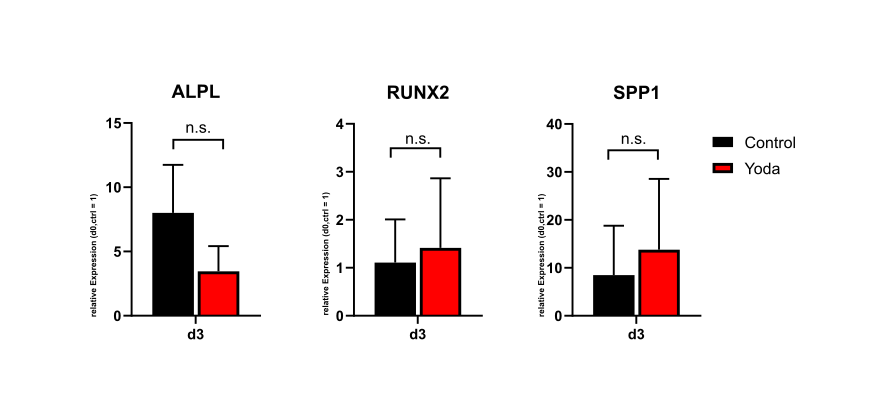
\includegraphics[width = \linewidth]{Osteogenic_PCR_Yoda.png}
	\caption{mRNA transcript levels of different late and early osteogenic markers, comparing cells 3 days after 5\textmu{}M (Yoda) \Piezo{} agonist exposure for 30min compared to negative control. Normalization agains negative control samples, harvested directly after intervention ended (n=3, Student's two-sided t-test).}
	\label{fig:Osteo_PCR}
\end{figure}
 

The tendency of our results 

One central aspect of Sugimoto's study was a certain "sweetspot" of hydrostatic pressure, after which increasing pressure would lead to insignificant results.



\section{Excursion: Biostability of \Yoda{} and \Piezo{} mediated apoptosis}
\label{sec:biostability}


\begin{figure}
	\centering
	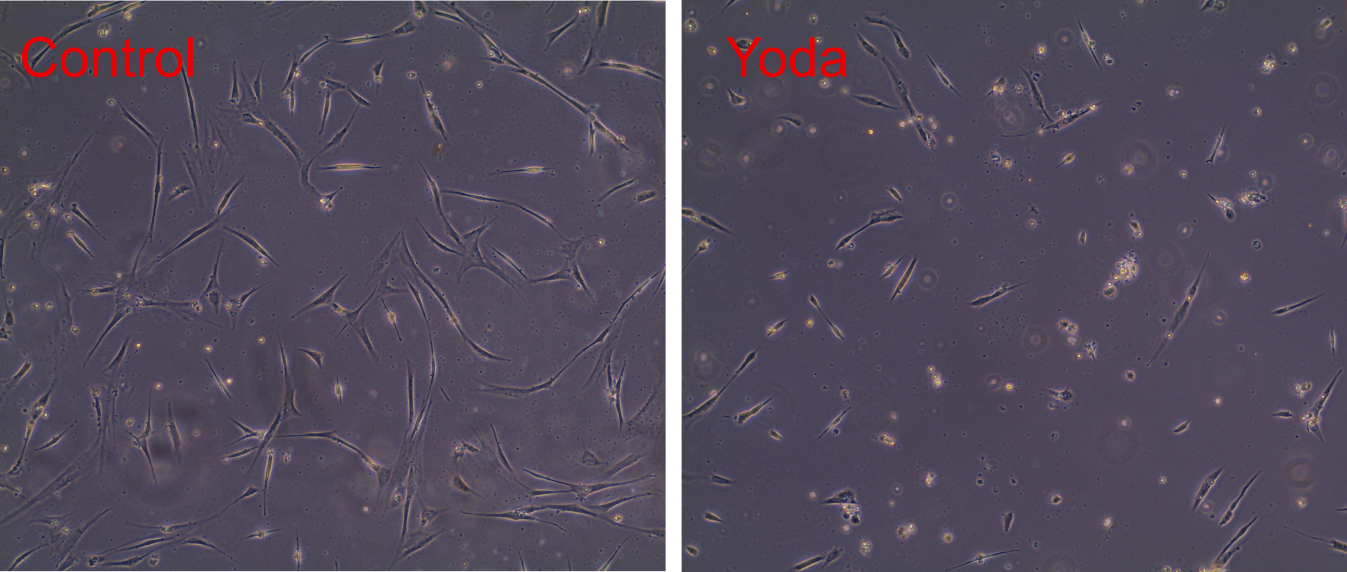
\includegraphics[width = \linewidth]{Yoda_Apoptosis.png}
	\caption{Light microscopy picture of serum-starved cells 7 days after intervention with either 0\textmu{}M (negative Control) or 5\textmu{}M (Yoda) chemical \Piezo{}-agonist.}
	\label{pic:Yoda_Apop}
\end{figure}

We realised there was a continous and large decrease in cell count in \Yoda{}-treated cells (see \ref{pic:Yoda_Apop}). Next to \Piezo{} being implicated in this pro-apoptotic effect, an intrinsic cytotoxicity of \Yoda{} could also be an explanation. To test this hypothesis, Uli, in an explorative experiment, exposed both \Piezo{}-KO and NoT Cell Lines to \Yoda{} similar to the one described ~\vref{sec:ChemicalStimulation}. Subsequent analysis suggested an apoptotic effect mediated through \Piezo{}. While there were no further investigations done, there are suggestions that calpain activation, downstream of \Piezo{}, has pro-apoptotic effects through caspase-3 and caspase-12 \cite{Nakagawa2000, Altznauer2004}. Furthermore, there is evidence that relates different intracellular calcium concentration to a set of cellular mechanisms, including cell migration and apoptosis. Here it might be worthwhile, to alter experimental \Yoda{} concentration to explore different regions of the continous cellular process spectrum. Another thing to keep in mind is that \Yoda{} activity might not only vary with concentration but also with time.
Our observations suggested that in standard incubation conditions \Yoda{} is transformed and looses its effect over time. (not shown) To test this hypothesis, we conducted an experiment similar to the one described in \ref{sec:ChemicalStimulation} only modifying the intervention medium. All the media was pre-incubated for 8 hours before intervention and either supplemented with 5\textmu{}M \Yoda{} before pre-incubation (8 hours Incubation) or directly after pre-incubation (No Incubation) or no \Yoda{} at all (Control). We found that incubation of \Yoda{} during a certain amount of time diminishes its bioactivity completely. This has not been published knowledge, but should be considered in future study designs. \myworries{Need to find long Yoda-Incubation paper.}



\begin{figure}
	\centering
	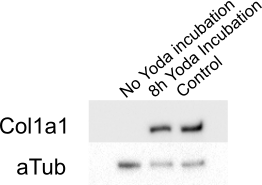
\includegraphics[width = \linewidth{}]{Inkubationshypothese.png}
	\caption{}
	\label{fig:Inkubationshypothese_Western}
\end{figure}